\chapter{Methodology}
\label{chapter:methodology}
In the thesis the main focus is to design a high linear, decoupled, modal structured multiaxial force sensors.
In the \nameref{chapter:literature_review} we describe theoretical background for the
task. 

The chapter specifies methodology of the design, therefore the chapter is divided into several sections. The first the \nameref{section:optical_modeling} section 
defines transition function for pressure sensor cell. The second section \nameref{section:calibration_pressure} describes the calibration method, used for pressure measurement cells.
\subfile{chapters/methodology/optical_modeling.tex}
\subfile{chapters/methodology/calibration_pressure.tex}
\section{Electric Design}
\begin{figure}[H]
  \centering
  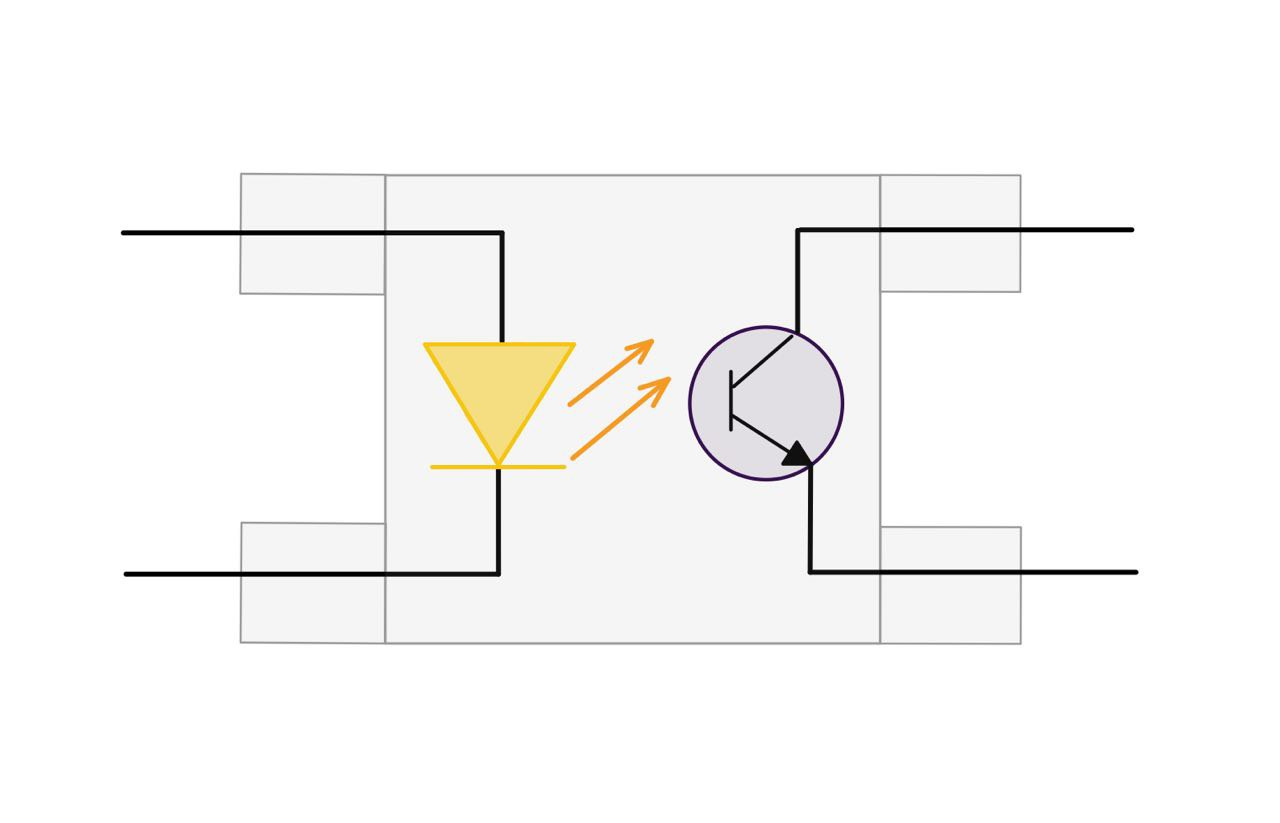
\includegraphics[width=\textwidth]{ED/optopair_scheme.jpg}
  \label{fig:optopair_scheme}
  \caption{General design of optopair sensor.}
\end{figure}

